\documentclass[11pt]{article}
\usepackage[T1]{fontenc}
\usepackage{lmodern}
\usepackage[margin=1in]{geometry}
\usepackage{amsmath,amssymb,amsthm}
\usepackage{microtype}
\usepackage{flafter}
\usepackage{enumitem}
\usepackage{tikz}
\usetikzlibrary{arrows.meta,positioning}
\usepackage[colorlinks=true,linkcolor=blue!45!black,citecolor=blue!45!black,urlcolor=blue!45!black]{hyperref}
\hypersetup{pdftitle={A superquadratic separation between sensitivity and block sensitivity}}
\newcommand{\bs}{\operatorname{bs}}
\newcommand{\unverified}[1]{\par\smallskip\noindent\fbox{\parbox{0.95\linewidth}{\textbf{Unverified step.} #1}}\par\smallskip}
\newtheorem{theorem}{Theorem}[section]
\newtheorem{lemma}[theorem]{Lemma}
\newtheorem{proposition}[theorem]{Proposition}
\newtheorem{corollary}[theorem]{Corollary}
\theoremstyle{definition}
\newtheorem{definition}[theorem]{Definition}
\theoremstyle{remark}
\newtheorem{remark}[theorem]{Remark}
\title{A superquadratic separation between sensitivity\\and block sensitivity}
\author{Rewritten for readability from the OpenAI manuscript of the same title}
\date{September 25, 2026}
\begin{document}
\maketitle
\begin{abstract}
We disprove the quadratic strengthening of the Sensitivity Conjecture by
constructing nonconstant total Boolean functions whose block sensitivity grows
faster than any constant multiple of sensitivity squared. In fact, for some
fixed \(\alpha>2\), the examples have unbounded block sensitivity and satisfy
\(\bs(f)\ge s(f)^\alpha\).
\end{abstract}

\section{The result}
\label{sec:introduction}

\subsection{Definitions and main theorem}

For a positive integer $n$ write $[n]=\{1,\ldots,n\}$. For
$x\in\{0,1\}^n$ and $B\subseteq[n]$, let $x^B$ be $x$ with exactly the
coordinates in $B$ flipped, and write $x^e=x^{\{e\}}$. Let
$f:\{0,1\}^n\to\{0,1\}$ be a total Boolean function, that is, one defined on
all of $\{0,1\}^n$.
\begin{itemize}[nosep]
\item \emph{Sensitivity:}
$s(f,x)=\bigl|\{e\in[n]:f(x^e)\ne f(x)\}\bigr|$ and $s(f)=\max_x s(f,x)$.
\item \emph{Block sensitivity:} a nonempty $B\subseteq[n]$ is a
\emph{sensitive block at $x$} if $f(x^B)\ne f(x)$. Then $\bs(f,x)$ is the
largest number of pairwise disjoint sensitive blocks at $x$, and
$\bs(f)=\max_x\bs(f,x)$.
\end{itemize}

\begin{theorem}\label{thm:main}
For every real \(C>0\), there are a positive integer \(n\) and a
nonconstant total Boolean function \(f:\{0,1\}^n\to\{0,1\}\) such that
\[
 \bs(f)>C\,s(f)^2.
\]
More precisely, for every integer \(d\ge1\) the construction below gives
a nonconstant total Boolean function \(f\) with
\[
 \frac{\bs(f)}{s(f)^2}\ge \frac{2^d}{4(d+2)^2}.
\]
\end{theorem}

Corollary~\ref{cor:power-separation} upgrades this to
$\bs(F_m,0)\ge s(F_m)^\alpha$ for a fixed $\alpha>2$ and a sequence $F_m$
with unbounded block sensitivity.

\paragraph{Background.}
Whether block sensitivity is bounded by a polynomial in sensitivity was the
Sensitivity Conjecture. It goes back to Nisan's work on parallel computation,
which introduced block sensitivity and recorded Rubinstein's quadratic
separation \cite[Section~2]{Nisan1989}, \cite{Rubinstein1995}. Nisan and
Szegedy suggested $\bs(f)\le s(f)^2$ \cite[Section~4]{NisanSzegedy1994}.
Virza obtained $\bs(f)=\tfrac12s(f)^2+\tfrac12s(f)$ \cite{Virza2011}, and
Ambainis and Sun $\bs(f)=\tfrac23s(f)^2-\tfrac13s(f)$
\cite[Theorem~1]{AmbainisSun2011}, which left a universal quadratic bound
open. Huang's degree bound with Tal's refinement \cite{Tal2013} gives
$\bs(f)\le s(f)^4$ \cite[Theorem~1.5]{Huang2019}, and Wellens proved
$\bs(f)\le\sqrt{2/3}\,s(f)^4+1$ \cite[Corollary~4.2]{Wellens2022}.
Theorem~\ref{thm:main} rules out the quadratic strengthening. The
construction adapts the tournament-indexed rows and selected blocking
coordinates of Meiburg's spectral-sensitivity construction
\cite[Sections~3.1 and~5.2--5.5]{Meiburg2026},\footnote{In the attribution
accompanying that construction, Meiburg credits GPT-5.6-Sol with the
gated-tournament ideas and describes his own contributions as exposition,
size and parameter optimization, and checking the faithfulness of the Lean
formalization.} with a different forbidden-label condition. Spectral
sensitivity $\lambda(f)$ \cite{AaronsonEtAl2021} satisfies
$\lambda(f)\le s(f)$, so a lower bound on $\bs(f)/\lambda(f)^2$ alone would
not give Theorem~\ref{thm:main}; no spectral input is used below. The final
OR step follows Ambainis and Sun \cite[Section~4, Lemma~1]{AmbainisSun2011}.
The amplification of a seed with $\bs>s^2$ by iteration was noted by Ambainis
and Pr\={u}sis \cite[Section~1]{AmbainisPrusis2014} and is an instance of the
composition method of Tal~\cite{Tal2013}. None of these is used as a black
box: every step is proved here.

\subsection{Proof at a glance}

Fix a depth $d$ and a large parameter $M$; put $k=2M^2+1$ and
$r=\lceil\sqrt M\rceil$.

\emph{Construction (Section~\ref{sec:construction}).}
For each level $\ell=0,\ldots,d$ we define predicates
$P_{\ell,1}\ge P_{\ell,2}\ge\cdots$ (pointwise; ``nested''). At level $0$
they are indicators of unions of Hamming balls of radii $d,d-1,\ldots,0$
around $M$ far-apart centres. A level-$\ell$ input is a $k\times r$ array of
level-$(\ell-1)$ inputs (``children''). The $k$ rows are the vertices of a
tournament with all outdegrees $M^2$, and each edge $i\to j$ carries a label
$a(i,j)\in[r]$ pointing at one child of row $j$. The predicate $P_{\ell,q}$
accepts when some \emph{clause} $i$ holds: the strongest child predicate
accepts every child of row $i$ (\emph{targets}), and a weaker child
predicate, depending on $q$, rejects the labelled child in each row $j$ with
$i\to j$ (\emph{gates}).

\emph{Many blocks (Lemma~\ref{lem:blocks}).} At the all-zero input, switching
on one row satisfies a clause, so the number of disjoint sensitive blocks is
multiplied by $k>2M^2$ per level.

\emph{Few sensitive bits (Proposition~\ref{prop:recurrences}).}
Let $S_{\ell,b}$ bound the number of single-bit flips taking a level-$\ell$
predicate from $b$ to $1-b$, and let $J_{\ell,b}$ bound the flips that move
\emph{two distinct} predicates from $b$ to $1-b$ at once. Then
\[
 S_{\ell,1}\le M^2S_{\ell-1,0}+rS_{\ell-1,1},\qquad
 S_{\ell,0}\le 16S_{\ell-1,0}+S_{\ell-1,1}+3J_{\ell-1,1}.
\]
For the first, fix one true clause; a flip must break one of its $M^2$ gates
or $r$ targets. The second is the heart of the proof. A flip from $0$ to $1$
must complete a clause that currently fails exactly one condition. The labels
(Lemma~\ref{lem:labelling}) allow at most $15$ clauses missing one target.
The tournament allows at most $3$ clauses missing one gate, and all but one
of these can be completed only by a flip changing two child predicates
simultaneously. The $J$'s obey similar recurrences and vanish at level $0$
(Lemma~\ref{lem:base}), because one bit cannot cross two radii.

\emph{Bookkeeping (Section~\ref{sec:separation}).}
For $M\ge9^{d+1}$ the recurrences give $S_{\ell,b}\le2(d+2)M^{\ell+b}$
(Lemma~\ref{lem:quantitative-profiles}): sensitivity grows by a factor about
$M$ per level, blocks by more than $2M^2$. The OR $f$ of $M$ copies of
$P_{d,1}$ has $s(f)\le2(d+2)M^{d+1}$ and $\bs(f,0)\ge M^2k^d$, which is
Theorem~\ref{thm:main}. Composing the $d=9$ instance with itself
(Lemma~\ref{lem:composition}) gives Corollary~\ref{cor:power-separation}.

\emph{Dependencies.}
Lemma~\ref{lem:labelling} $\Rightarrow$ Proposition~\ref{prop:recurrences};
Lemma~\ref{lem:base} and Proposition~\ref{prop:recurrences} $\Rightarrow$
Lemma~\ref{lem:quantitative-profiles};
Lemmas~\ref{lem:blocks} and~\ref{lem:quantitative-profiles} $\Rightarrow$
Theorem~\ref{thm:main}; the $d=9$ case and Lemma~\ref{lem:composition}
$\Rightarrow$ Corollary~\ref{cor:power-separation}.

\emph{Notation changes from the source.} A coordinate is called $e$ (the
source's $a$ clashed with the labels $a(i,j)$). In
Lemma~\ref{lem:composition} the dimensions are $n_1,n_2$, the block counts
$p_1,p_2$ and the blocks $\Gamma_i,\Delta_j$, to avoid clashes with $q$, $b$,
$C$ and $E_j$.

\section{The labelled tournament and nested predicates}
\label{sec:construction}

\subsection{Parameters and labels}

Fix integers \(d\ge1\) and \(M\ge3\), and put
\[
 L=d+2,\qquad k=2M^2+1,\qquad r=\lceil\sqrt M\rceil,\qquad t=16.
\]
(Section~\ref{sec:separation} takes $M\ge9^{d+1}$.) A \emph{tournament} on
$[k]$ contains, for each pair of distinct $i,j\in[k]$, exactly one of the
directed edges $i\to j$, $j\to i$. Fix one in which every vertex has
outdegree $M^2$. One exists: identify $[k]$ with $\mathbb Z/k$ and let
$i\to j$ when $j-i\in\{1,\ldots,M^2\}$ modulo $k$; since $k=2M^2+1$, exactly
one of $j-i$ and $i-j$ lies in that range.

\begin{lemma}\label{lem:labelling}
The edges can be labelled by numbers \(a(i,j)\in[r]\), one for each edge
$i\to j$, so that there is no set \(I\subseteq[k]\) of size \(t\) admitting
choices \(m_j\in[r]\), \(j\in I\), with
\[
 a(i,j)=m_j \qquad\text{for every edge }i\to j\text{ within }I.
\]
\end{lemma}
This is used only to bound $|\mathcal T|$ in Step~4 of
Proposition~\ref{prop:recurrences}.
\begin{proof}
Choose all labels independently and uniformly from $[r]$. Call a pair
$(I,(m_j)_{j\in I})$ a \emph{pattern}; it is \emph{realised} if all the
displayed equalities hold.

\emph{One pattern.} There are $\binom{16}{2}=120$ edges within $I$. Each
edge $i\to j$ imposes one equation $a(i,j)=m_j$ on its own label, which holds
with probability $1/r$. Labels of different edges are independent, so the
pattern is realised with probability $r^{-120}$.

\emph{Union bound.} There are at most $k^{16}$ sets $I$ and $r^{16}$ choices
of $(m_j)$. Hence
\[
 \Pr[\text{some pattern is realised}]
 \le k^{16}r^{16}r^{-120}=k^{16}r^{-104}
 \le(3M^2)^{16}(\sqrt M)^{-104}=3^{16}M^{-20}\le3^{-4}<1,
\]
using $k\le3M^2$, $r\ge\sqrt M$, $M^{32-52}=M^{-20}$ and $M\ge3$. So some
labelling realises no pattern.
\end{proof}

Fix such a labelling from now on.

\subsection{The predicates}

For \(0\le\ell\le d\), set
\[
 H_\ell=d+1-\ell,\qquad N_\ell=LM(kr)^\ell.
\]
We define $P_{\ell,q}:\{0,1\}^{N_\ell}\to\{0,1\}$ for $1\le q\le H_\ell$ by
recursion on $\ell$.

\paragraph{Level $0$.}
Partition $[LM]$ into blocks $E_1,\ldots,E_M$ of size $L$, and let
$z_j\in\{0,1\}^{LM}$ be the indicator of $E_j$ (the \emph{centres}). With
$\operatorname{dist}$ the Hamming distance, set
\[
 D(x)=\min_{j\in[M]}\operatorname{dist}(x,z_j),\qquad
 P_{0,q}(x)=\mathbf1\{D(x)\le d+1-q\}\quad(1\le q\le d+1).
\]
The radii $d+1-q$ run through $d,d-1,\ldots,0$; distinct centres are at
distance $2L=2d+4$.

\paragraph{Level $\ell\ge1$.}
Put $H=H_\ell$ and $Q=H+1=H_{\ell-1}$, so $Q$ is the largest index at level
$\ell-1$. Split $x\in\{0,1\}^{N_\ell}$ into $kr$ disjoint \emph{children}
$x_{j,c}\in\{0,1\}^{N_{\ell-1}}$, with row $j\in[k]$ and position $c\in[r]$;
this matches $N_\ell=krN_{\ell-1}$. For $i\in[k]$ and $q\in[H]$, say that
\emph{clause $i$ holds at index $q$} (at $x$) if
\begin{equation}\label{eq:predicate-definition}
 \begin{aligned}
 P_{\ell-1,Q}(x_{i,c})&=1 &&\text{for all }c\in[r]
   &&\text{(\emph{target conditions})},\\
 P_{\ell-1,Q-q}(x_{j,a(i,j)})&=0 &&\text{for all $j$ with }i\to j
   &&\text{(\emph{gate conditions})}.
 \end{aligned}
\end{equation}
Define $P_{\ell,q}(x)=1$ if some clause holds at index $q$, and $0$
otherwise. The indices are valid because $1\le Q-q\le H<Q$. A clause has $r$
targets and $M^2$ gates; the targets do not depend on $q$, and the child
tested by each gate does not depend on $q$.

\begin{figure}[htbp]
\centering
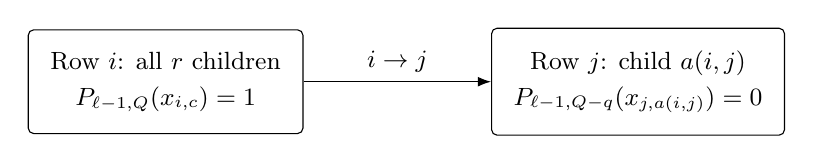
\begin{tikzpicture}[>=Latex, every node/.style={font=\small},
  condition/.style={draw,rounded corners=2pt,inner sep=8pt,align=center}]
 \node[condition] (target) at (0,0)
   {Row \(i\): all \(r\) children\\[2pt]
    \(P_{\ell-1,Q}(x_{i,c})=1\)};
 \node[condition] (gate) at (6,0)
   {Row \(j\): child \(a(i,j)\)\\[2pt]
    \(P_{\ell-1,Q-q}(x_{j,a(i,j)})=0\)};
 \draw[->] (target) -- node[above]{\(i\to j\)} (gate);
\end{tikzpicture}
\caption{Clause $i$: one target per child of row $i$, one gate per
out-neighbour $j$. Raising $q$ strengthens the gates only.}
\label{fig:clause}
\end{figure}

Two facts are used throughout.

\paragraph{(N) Nesting.}
\emph{For every level $\ell$, input $x$ and indices $p<p'$: if
$P_{\ell,p'}(x)=1$ then $P_{\ell,p}(x)=1$; equivalently, if
$P_{\ell,p}(x)=0$ then $P_{\ell,p'}(x)=0$. For $\ell\ge1$, a clause holding
at index $p'$ also holds at index $p$.}

\emph{Proof by induction on $\ell$.} At level $0$, $D(x)\le d+1-p'$ implies
$D(x)\le d+1-p$. Let $\ell\ge1$ and let clause $i$ hold at index $p'$. Its
targets are the same at index $p$. For each gate child $y$ we have
$P_{\ell-1,Q-p'}(y)=0$ and $Q-p'<Q-p$, so (N) at level $\ell-1$ gives
$P_{\ell-1,Q-p}(y)=0$. Hence clause $i$ holds at index $p$, and
$P_{\ell,p}(x)=1$. \qed

Nesting concerns the predicate index, not the input bits: the smallest index
is the easiest to satisfy.

\paragraph{(SC) One flip, one condition.}
\emph{Fix $\ell\ge1$, an index $q$ and a clause $i$. Flipping one coordinate
$e\in[N_\ell]$ changes the truth value of at most one condition of clause $i$
at index $q$.}

\emph{Proof.} The $r+M^2$ conditions test pairwise distinct children: the
targets are the $r$ children of row $i$; each gate tests a child in a row
$j\ne i$, and distinct gates use distinct rows because there is only one
edge between $i$ and $j$. The coordinate $e$ lies in exactly one child. \qed

The same flip may affect many clauses and several predicates of its child;
the counts below are unions over clauses.

\subsection{Sensitivity profiles and the initial bounds}

For $b\in\{0,1\}$ and $0\le\ell\le d$ define
\begin{align*}
 S_{\ell,b}&=\max_{\substack{1\le q\le H_\ell,\ x\\ P_{\ell,q}(x)=b}}
 \bigl|\{e\in[N_\ell]:P_{\ell,q}(x^e)=1-b\}\bigr|,\\
 J_{\ell,b}&=\max_{\substack{1\le q<q'\le H_\ell,\ x\\
                         P_{\ell,q}(x)=P_{\ell,q'}(x)=b}}
 \bigl|\{e\in[N_\ell]:P_{\ell,q}(x^e)=P_{\ell,q'}(x^e)=1-b\}\bigr|.
\end{align*}
A maximum over no cases is zero; in particular $J_{d,0}=J_{d,1}=0$, since
$H_d=1$. In $J$, both predicates are evaluated at the same input and changed
by the same flip.

\begin{lemma}\label{lem:base}
The initial sensitivity profiles satisfy
\begin{equation}\label{eq:base-profile}
 S_{0,0}\le L,\qquad S_{0,1}\le LM,\qquad J_{0,0}=J_{0,1}=0.
\end{equation}
\end{lemma}
This is the base case of Lemma~\ref{lem:quantitative-profiles}.
\begin{proof}
\emph{(i) $|D(x)-D(x^e)|\le1$.} For each $j$, the distances
$\operatorname{dist}(x,z_j)$ and $\operatorname{dist}(x^e,z_j)$ differ by
exactly $1$, so the minima over $j$ differ by at most $1$.

\emph{(ii) $S_{0,0}\le L$.} Fix $q$, put $R=d+1-q\in\{0,\ldots,d\}$, and let
$D(x)>R$. Suppose $D(x^e)\le R$, and pick a centre $z_j$ with
$\operatorname{dist}(x^e,z_j)\le R$. Then
$\operatorname{dist}(x,z_j)\le R+1\le d+1$. At most one centre lies within
distance $d+1$ of $x$, because two such centres would be at distance at most
$2d+2<2L$ by the triangle inequality. So $z_j$ is the same centre $z$ for
every such $e$. Since $\operatorname{dist}(x,z)\ge D(x)\ge R+1$, we get
$\operatorname{dist}(x,z)=R+1$, and the flip must decrease this distance:
$e$ is one of the $R+1$ coordinates where $x$ and $z$ differ. Thus there are
at most $R+1\le d+1\le L$ such $e$.

\emph{(iii) $S_{0,1}\le LM$}, the number of coordinates.

\emph{(iv) $J_{0,b}=0$.} Let $q<q'$, with integer radii $R=d+1-q>R'=d+1-q'$.
If a flip took both predicates from $0$ to $1$, then
$D(x)>R\ge R'+1$, so $D(x)\ge R'+2$, while $D(x^e)\le R'$; this contradicts
(i). If a flip took both from $1$ to $0$, then $D(x)\le R'$ and
$D(x^e)\ge R+1\ge R'+2$, again contradicting (i).
\end{proof}

\subsection{Disjoint blocks at zero}
\begin{lemma}\label{lem:blocks}
At every level \(0\le\ell\le d\), all predicates are zero at the
all-zero input. There are \(Mk^\ell\) pairwise disjoint nonempty blocks
of coordinates, each of size \(Lr^\ell\), such that flipping any one
block at zero makes every predicate at that level equal to one.
\end{lemma}
This gives the block-sensitivity lower bound in the proof of
Theorem~\ref{thm:main}.
\begin{proof}
Induction on $\ell$.

\emph{Level $0$.} Each centre has weight $L$, so $D(0)=L>d$ and every
$P_{0,q}(0)=0$. The $M$ blocks $E_j$ have size $L$, and $0^{E_j}=z_j$ has
$D=0$, so every $P_{0,q}(z_j)=1$.

\emph{Level $\ell\ge1$.} Let $B_1,\ldots,B_{Mk^{\ell-1}}$ be the blocks at
level $\ell-1$. At the all-zero input every child is all-zero, so
$P_{\ell-1,Q}=0$ on every child by induction; every clause fails a target,
and every $P_{\ell,q}(0)=0$.

For a row $i$ and an index $h$, let $U_{i,h}$ be the union over $c\in[r]$ of
the copy of $B_h$ inside child $(i,c)$. After flipping $U_{i,h}$ at zero,
every child of row $i$ equals $0^{B_h}$ and all other children are
all-zero. By induction $P_{\ell-1,Q}(0^{B_h})=1$, so the targets of clause
$i$ hold. Each gate child of clause $i$ lies in another row, is all-zero, and
so has $P_{\ell-1,Q-q}=0$ by induction; the gates hold for every $q$. Hence
every $P_{\ell,q}$ equals $1$ after the flip.

The sets $U_{i,h}$ are pairwise disjoint: for different rows they lie in
different children, and for the same row they are disjoint inside each child
because the $B_h$ are disjoint. There are $k\cdot Mk^{\ell-1}=Mk^\ell$ of
them, each of size $r\cdot Lr^{\ell-1}=Lr^\ell$.
\end{proof}

\section{Sensitivity recurrences}
\label{sec:recurrences}

\begin{proposition}\label{prop:recurrences}
For $1\leq \ell\leq d$, write
$S'_b=S_{\ell-1,b}$ and $J'_b=J_{\ell-1,b}$.  Then
\begin{equation}\label{eq:recurrences}
\begin{aligned}
 S_{\ell,1}&\leq M^2S'_0+rS'_1,
 &\qquad J_{\ell,1}&\leq M^2J'_0+rS'_1,\\
 S_{\ell,0}&\leq tS'_0+S'_1+3J'_1,
 &\qquad J_{\ell,0}&\leq tS'_0+3J'_1.
\end{aligned}
\end{equation}
\end{proposition}
These four inequalities feed Lemma~\ref{lem:quantitative-profiles}. They hold
at every input, not only near the all-zero input.

\begin{proof}
\emph{Plan.} On the one-side (Steps 1--2) we fix one true clause and count
the flips that break it. On the zero-side (Steps 3--7) we show that only
boundedly many clauses can be completed by a single flip, and count the
flips completing each.

\emph{Step 0: conventions.} Fix $\ell$, $H=H_\ell$, $Q=H+1$. A \emph{flip} is
a flip of one coordinate $e\in[N_\ell]$; it lies in one child $y$. By the
definitions of $S'_b$ and $J'_b$, applied to $y$:
\begin{itemize}[nosep]
\item[(C1)] for a fixed child $y$ and index $p$, at most $S'_b$ flips change
$P_{\ell-1,p}(y)$ from $b$ to $1-b$;
\item[(C2)] for a fixed child $y$ and indices $p\ne p'$, at most $J'_b$ flips
change both $P_{\ell-1,p}(y)$ and $P_{\ell-1,p'}(y)$ from $b$ to $1-b$.
\end{itemize}

\emph{Step 1: $S_{\ell,1}\le M^2S'_0+rS'_1$.}
Fix $q$ and $x$ with $P_{\ell,q}(x)=1$, and fix one clause $i$ holding at
index $q$ at $x$. If $P_{\ell,q}(x^e)=0$, then clause $i$ fails at $x^e$, so
the flip makes one of its conditions false. Either $P_{\ell-1,Q}$ changes
from $1$ to $0$ on one of the $r$ target children (at most $S'_1$ flips each,
by (C1)), or $P_{\ell-1,Q-q}$ changes from $0$ to $1$ on one of the $M^2$
gate children (at most $S'_0$ flips each).

\emph{Step 2: $J_{\ell,1}\le M^2J'_0+rS'_1$.}
Fix $q<q'$ and $x$ with $P_{\ell,q}(x)=P_{\ell,q'}(x)=1$. Fix one clause $i$
holding at index $q'$ at $x$; by (N) it also holds at index $q$. Put
\[
 g=Q-q,\qquad g'=Q-q',\qquad 1\le g'<g<Q.
\]
Let $e$ be a flip after which both parent predicates are $0$. Then clause $i$
fails at index $q$ at $x^e$.

\emph{Case A: a target of clause $i$ fails at $x^e$.} As in Step 1, at most
$rS'_1$ flips.

\emph{Case B: all targets hold at $x^e$.} Then some gate of clause $i$ fails
at index $q$: its child $y$ has $P_{\ell-1,g}=1$ after the flip, hence
$P_{\ell-1,g'}=1$ after the flip by (N). Before the flip, $P_{\ell-1,g'}(y)=0$
because clause $i$ held at index $q'$, hence $P_{\ell-1,g}(y)=0$ by (N). So
the flip changes the two distinct predicates $P_{\ell-1,g'}$ and
$P_{\ell-1,g}$ on $y$ from $0$ to $1$. By (C2) there are at most $J'_0$ such
flips for each of the $M^2$ gate children.

\emph{Step 3: candidate clauses at a zero.}
Fix $q$ and $x$ with $P_{\ell,q}(x)=0$. Let $\mathcal T$ be the set of
$i\in[k]$ whose clause, at index $q$ at $x$, fails exactly one target and no
gate, and $\mathcal G$ the set of $i$ whose clause fails exactly one gate
and no target. Both sets depend only on $(x,q)$, not on any flip.

\emph{Claim.} If clause $i$ holds at index $q$ at $x^e$, then
$i\in\mathcal T\cup\mathcal G$ and the flip changes the unique failed
condition of clause $i$ from false to true.

Indeed, clause $i$ is false at $x$, since $P_{\ell,q}(x)=0$, and true at
$x^e$. By (SC) at most one of its conditions changed, so exactly one was
false at $x$, and that one was repaired.

\emph{Step 4: $|\mathcal T|\le t-1$.}
For $j\in\mathcal T$ let $m_j\in[r]$ be the position of its unique failed
target, so $P_{\ell-1,Q}(x_{j,c})=0$ exactly when $c=m_j$. Let
$i,j\in\mathcal T$ with $i\to j$. Clause $i$ fails no gate, so
$P_{\ell-1,Q-q}(x_{j,a(i,j)})=0$. Since $Q-q<Q$, (N) gives
$P_{\ell-1,Q}(x_{j,a(i,j)})=0$. Thus position $a(i,j)$ is a failed target of
clause $j$, which forces $a(i,j)=m_j$. If $|\mathcal T|\ge t$, any
$t$-element $I\subseteq\mathcal T$ with these $m_j$ would contradict
Lemma~\ref{lem:labelling}.

\emph{Step 5: $|\mathcal G|\le3$, with at most one exceptional vertex.}
For $j\in\mathcal G$ every child of row $j$ has $P_{\ell-1,Q}=1$. Let
$i,j\in\mathcal G$ with $i\to j$. The gate child $x_{j,a(i,j)}$ of clause
$i$ lies in row $j$, so $P_{\ell-1,Q}=1$ there, and (N) gives
$P_{\ell-1,Q-q}=1$ there: this gate of clause $i$ fails. Clause $i$ fails
only one gate, so every vertex of $\mathcal G$ has at most one out-neighbour
in $\mathcal G$. With $m=|\mathcal G|$, counting the edges within
$\mathcal G$ by their tails gives
\[
 \frac{m(m-1)}2\le m,\qquad\text{hence}\qquad m\le3.
\]
Of any two vertices of $\mathcal G$, one has an edge to the other. So at most
one vertex of $\mathcal G$ has no out-neighbour in $\mathcal G$; call it
\emph{exceptional} if it exists.

\emph{Step 6: $S_{\ell,0}\le tS'_0+S'_1+3J'_1$.}
By Step 3, every flip with $P_{\ell,q}(x^e)=1$ repairs the unique failed
condition of some $i\in\mathcal T\cup\mathcal G$. We bound the number of such
flips for each $i$.
\begin{itemize}[nosep]
\item $i\in\mathcal T$: the flip changes $P_{\ell-1,Q}$ on child $x_{i,m_i}$
from $0$ to $1$; at most $S'_0$ flips by (C1). Total at most $(t-1)S'_0$ by
Step 4.
\item $i\in\mathcal G$ not exceptional, say $i\to j$ with $j\in\mathcal G$:
by Step 5 the unique failed gate of clause $i$ is at $y=x_{j,a(i,j)}$, where
before the flip $P_{\ell-1,Q-q}(y)=P_{\ell-1,Q}(y)=1$. The repair makes
$P_{\ell-1,Q-q}(y)=0$, hence $P_{\ell-1,Q}(y)=0$ by (N). The indices $Q-q$
and $Q$ are distinct, so by (C2) there are at most $J'_1$ such flips. (The
flip breaks a target of clause $j$; this is harmless, since the accepting
clause is $i$, whose targets and other gates are untouched.)
\item $i$ exceptional: the flip changes $P_{\ell-1,Q-q}$ on one fixed child
from $1$ to $0$; at most $S'_1$ flips.
\end{itemize}
Since $|\mathcal G|\le3$, the total is at most $(t-1)S'_0+S'_1+3J'_1$.

\emph{Step 7: $J_{\ell,0}\le tS'_0+3J'_1$.}
Fix $q<q'$ and $x$ with $P_{\ell,q}(x)=P_{\ell,q'}(x)=0$. Form $\mathcal T$
and $\mathcal G$ as in Step 3 for the \emph{smaller} index $q$, and let
$g,g'$ be as in Step 2. Let $e$ be a flip after which both parent predicates
are $1$. Choose a clause $i$ holding at index $q'$ at $x^e$; the choice may
depend on $e$. By (N) it holds at index $q$ at $x^e$, so by Step 3
$i\in\mathcal T\cup\mathcal G$ and $e$ repairs its unique failed condition at
index $q$.
\begin{itemize}[nosep]
\item $i\in\mathcal T$: at most $S'_0$ flips per clause as in Step 6, in
total at most $(t-1)S'_0$.
\item $i\in\mathcal G$, exceptional or not: the unique failed gate at index
$q$ is at a child $y$ with $P_{\ell-1,g}(y)=1$ before the flip, so
$P_{\ell-1,g'}(y)=1$ before the flip by (N). After the flip clause $i$ holds
at index $q'$, and its gate for the same edge tests the same child, so
$P_{\ell-1,g'}=0$ on $y$, hence $P_{\ell-1,g}=0$ by (N). Both distinct
predicates change from $1$ to $0$: at most $J'_1$ flips by (C2), and at most
$3J'_1$ in total by Step 5. No target value at $y$ is needed here; the second
parent index supplies the second child predicate.
\end{itemize}
Every counted flip falls under one of these cases, so
$J_{\ell,0}\le tS'_0+3J'_1$.

All bounds hold for each admissible $x$ and each index or pair of indices, so
they hold for the maxima. If $H=1$ there are no pairs $q<q'$, and the two
joint inequalities hold because their left sides are zero.
\end{proof}

\section{Quantitative bounds and separation}
\label{sec:separation}

\begin{lemma}
\label{lem:quantitative-profiles}
Suppose that $d\geq 1$ and $M\geq 9^{d+1}$.
For every $0\leq\ell\leq d$ and $b\in\{0,1\}$, the predicates of the
construction satisfy
\[
  S_{\ell,b}\leq 2L M^{\ell+b}.
\]
\end{lemma}
It is used at $\ell=d$ in the proof of Theorem~\ref{thm:main}.

\begin{proof}
\emph{Plan.} Normalise $S_{\ell,b}$ and $J_{\ell,b}$ by $M^{\ell+b}$. This
turns~\eqref{eq:recurrences} into a two-term linear recurrence with a small
parameter $\epsilon$, which is solved by induction.

\emph{Step 1: normalisation.} Define
\[
 u_\ell=\max_{b\in\{0,1\}}\frac{S_{\ell,b}}{M^{\ell+b}},
 \qquad
 v_\ell=\max_{b\in\{0,1\}}\frac{J_{\ell,b}}{M^{\ell+b}},
 \qquad
 \epsilon=\frac{\max(r,t)}{M}.
\]
By~\eqref{eq:base-profile}, $u_0\le\max(L,LM/M)=L$ and $v_0=0$.

\emph{Step 2: normalised recurrences.} Let $1\le\ell\le d$ and write
$u=u_{\ell-1}$, $v=v_{\ell-1}$. By definition $S'_0\le uM^{\ell-1}$,
$S'_1\le uM^\ell$, $J'_0\le vM^{\ell-1}$ and $J'_1\le vM^\ell$. Substituting
into~\eqref{eq:recurrences}:
\begin{align*}
 S_{\ell,1}&\le M^2uM^{\ell-1}+ruM^\ell
   =\Bigl(1+\frac rM\Bigr)u\,M^{\ell+1},
 &S_{\ell,0}&\le tuM^{\ell-1}+uM^\ell+3vM^\ell
   =\Bigl(\Bigl(1+\frac tM\Bigr)u+3v\Bigr)M^\ell,\\
 J_{\ell,1}&\le M^2vM^{\ell-1}+ruM^\ell
   =\Bigl(\frac rMu+v\Bigr)M^{\ell+1},
 &J_{\ell,0}&\le tuM^{\ell-1}+3vM^\ell
   =\Bigl(\frac tMu+3v\Bigr)M^\ell.
\end{align*}
Since $r/M,t/M\le\epsilon$ and $v\le3v$,
\begin{equation}
\label{eq:normalized-recurrences}
  u_\ell\leq (1+\epsilon)u_{\ell-1}+3v_{\ell-1},\qquad
  v_\ell\leq \epsilon u_{\ell-1}+3v_{\ell-1}.
\end{equation}

\emph{Step 3: size of $\epsilon$.} Since $M\ge9^{d+1}\ge81$, we have
$\sqrt M\ge9$, so $r=\lceil\sqrt M\rceil\le\sqrt M+1\le2\sqrt M$ and
$t=16\le2\sqrt M$. Hence
\begin{equation}
\label{eq:epsilon-choice}
 \epsilon\leq\frac{2}{\sqrt M}\leq\frac{2}{3^{d+1}}.
\end{equation}

\emph{Step 4: comparison sequences.} Let $U_0=L$, $V_0=0$ and
\[
 U_\ell=(1+\epsilon)U_{\ell-1}+3V_{\ell-1},
 \qquad
 V_\ell=\epsilon U_{\ell-1}+3V_{\ell-1}.
\]
The coefficients are nonnegative, so~\eqref{eq:normalized-recurrences} and
induction give $u_\ell\le U_\ell$ and $v_\ell\le V_\ell$. We claim that for
$0\le\ell\le d$
\begin{equation}
\label{eq:comparison-bounds}
 U_\ell\leq2L,
 \qquad
 V_\ell\leq\epsilon L(3^\ell-1).
\end{equation}
This holds at $\ell=0$. Assume it for all indices below some
$1\le\ell\le d$. First,
\[
 V_\ell\le2\epsilon L+3\epsilon L(3^{\ell-1}-1)=\epsilon L(3^\ell-1).
\]
Next, $U_j-U_{j-1}=\epsilon U_{j-1}+3V_{j-1}$, and summing these increments
gives
\begin{align*}
 U_\ell
 &=L+\sum_{j=0}^{\ell-1}(\epsilon U_j+3V_j)
 \le L+2\epsilon L\ell+3\epsilon L\sum_{j=0}^{\ell-1}(3^j-1)\\
 &=L+2\epsilon L\ell+3\epsilon L\Bigl(\frac{3^\ell-1}2-\ell\Bigr)
 =L+\epsilon L\Bigl[\frac32(3^\ell-1)-\ell\Bigr].
\end{align*}
By~\eqref{eq:epsilon-choice} and $\ell\le d$,
\[
 \epsilon\Bigl[\frac32(3^\ell-1)-\ell\Bigr]
 \le\frac{2}{3^{d+1}}\cdot\frac{3^{\ell+1}-3-2\ell}{2}
 =\frac{3^{\ell+1}-3-2\ell}{3^{d+1}}<1,
\]
so $U_\ell<2L$. This completes the induction. Finally
$S_{\ell,b}\le u_\ell M^{\ell+b}\le U_\ell M^{\ell+b}\le2LM^{\ell+b}$.
\end{proof}

\begin{proof}[Proof of Theorem~\ref{thm:main}]
Fix an integer $d\ge1$ and an integer $M\ge9^{d+1}$ (so $M\ge3$), and labels
as in Lemma~\ref{lem:labelling}. Following the OR-balancing principle of
Ambainis and Sun \cite[Section~4, Lemma~1]{AmbainisSun2011}, let $f$ be the
OR of $M$ copies of $P_{d,1}$ on disjoint sets of variables. It is a total
Boolean function on
\begin{equation}
\label{eq:final-dimension}
 n=M\cdot N_d=LM^2(kr)^d
\end{equation}
bits. Recall $H_d=1$, so $S_{d,b}$ refers to $P_{d,1}$ alone.

\emph{Step 1: $f(0)=0$ and $f$ is nonconstant.} By Lemma~\ref{lem:blocks},
each copy is $0$ at its all-zero input, and flipping one of its blocks makes
that copy, hence $f$, equal to $1$.

\emph{Step 2: sensitivity.} Let $f(x)=0$. Then every copy is $0$, and a flip
changes $f$ only if it turns its own copy to $1$; there are at most $S_{d,0}$
such flips in each of the $M$ copies. Let $f(x)=1$. If at least two copies
accept, no single flip makes $f$ zero. If exactly one accepts, a sensitive
flip must lie in that copy and turn it to $0$, giving at most $S_{d,1}$
flips. By Lemma~\ref{lem:quantitative-profiles},
\begin{equation}
\label{eq:final-sensitivity}
 s(f)\leq\max\{M S_{d,0},S_{d,1}\}
       \leq2L M^{d+1}.
\end{equation}

\emph{Step 3: block sensitivity.} By Lemma~\ref{lem:blocks}, each copy has
$Mk^d$ pairwise disjoint blocks, each of which turns that copy, hence $f$,
to $1$ when flipped at zero. Blocks in different copies are disjoint, so
\begin{equation}
\label{eq:final-block-sensitivity}
 \bs(f,0)\geq M^2k^d.
\end{equation}

\emph{Step 4: the ratio.} Since $f$ is nonconstant, $s(f)>0$. Using
$k/M^2>2$ and $L=d+2$,
\begin{equation}
\label{eq:ratio-separation}
 \frac{\bs(f)}{s(f)^2}
 \geq\frac{M^2k^d}{4L^2M^{2d+2}}
 =\frac{(k/M^2)^d}{4L^2}
 \geq\frac{2^d}{4(d+2)^2}.
\end{equation}
The right side tends to infinity with $d$. Given $C>0$, choose $d$ with
$2^d/(4(d+2)^2)>C$, then $M$, labels and $f$ as above; then
$\bs(f)>C\,s(f)^2$.
\end{proof}

\emph{Sanity check.} The bound $2^d/(4(d+2)^2)$ is $256/400<1$ at $d=8$ and
$512/484>1$ at $d=9$; this is why the corollary below uses $d=9$.

\subsection{A fixed exponent by composition}

\begin{lemma}
\label{lem:composition}
Let $f:\{0,1\}^{n_1}\to\{0,1\}$ and
$g:\{0,1\}^{n_2}\to\{0,1\}$ be total Boolean functions.
Their disjoint composition is the function on $n_1n_2$ bits defined by
\[
 (f\circ g)(x_1,\ldots,x_{n_1})
   =f\bigl(g(x_1),\ldots,g(x_{n_1})\bigr),
 \qquad x_i\in\{0,1\}^{n_2}.
\]
Then
\[
 s(f\circ g)\leq s(f)s(g).
\]
If $g(0)=0$, then $(f\circ g)(0)=f(0)$ and
\[
 \bs(f\circ g,0)\geq\bs(f,0)\bs(g,0).
\]
More explicitly, any disjoint families of $p_1$ and $p_2$ blocks sensitive at
zero for $f$ and $g$, respectively, yield a disjoint family of $p_1p_2$
blocks sensitive at zero for $f\circ g$.
\end{lemma}
This is the induction step in Corollary~\ref{cor:power-separation}.

\begin{proof}
\emph{Sensitivity.} Fix $x=(x_1,\ldots,x_{n_1})$ and put
$y=(g(x_1),\ldots,g(x_{n_1}))$. Flipping a coordinate $e$ of child $x_i$
replaces $y$ by $y^{i}$ if $g(x_i^e)\ne g(x_i)$ and leaves $y$ unchanged
otherwise. So $e$ is sensitive for $f\circ g$ at $x$ exactly when $e$ is
sensitive for $g$ at $x_i$ and $i$ is sensitive for $f$ at $y$. Therefore
\[
 s(f\circ g,x)
   =\sum_{i:\,f(y^{i})\ne f(y)}s(g,x_i)
   \leq s(f,y)s(g)
   \leq s(f)s(g).
\]

\emph{Blocks.} Let $g(0)=0$. At the all-zero input $y=0$, so
$(f\circ g)(0)=f(0)$. Let $\Gamma_1,\ldots,\Gamma_{p_1}\subseteq[n_1]$ and
$\Delta_1,\ldots,\Delta_{p_2}\subseteq[n_2]$ be pairwise disjoint sensitive
blocks at zero for $f$ and $g$. Identify the coordinates of $f\circ g$ with
$[n_1]\times[n_2]$ and consider the $p_1p_2$ sets $\Gamma_i\times\Delta_j$.
They are nonempty and pairwise disjoint, because the $\Gamma_i$ are disjoint
and the $\Delta_j$ are disjoint. Flipping $\Gamma_i\times\Delta_j$ at zero
turns each child indexed by $\Gamma_i$ into $0^{\Delta_j}$, where $g=1$, and
leaves the other children all-zero, where $g=0$. The outer input becomes
$0^{\Gamma_i}$, and $f(0^{\Gamma_i})\ne f(0)$. So each
$\Gamma_i\times\Delta_j$ is sensitive at zero. Taking maximum families gives
the inequality; it is trivial if either maximum is zero.
\end{proof}

\begin{corollary}
\label{cor:power-separation}
There exist a real number $\alpha>2$ and nonconstant total Boolean
functions $F_m$, for integers $m\geq1$, such that
\[
 \bs(F_m,0)\geq s(F_m)^\alpha
 \qquad\text{for every }m,
 \qquad
 \bs(F_m,0)\longrightarrow\infty.
\]
\end{corollary}

\begin{proof}
\emph{Seed.} Fix $d=9$, so $L=11$, an integer $M\ge9^{10}$ and admissible
labels, and let $f$ be the function from the proof of
Theorem~\ref{thm:main}. Put
\[
 A=22M^{10},\qquad B=M^2k^9.
\]
Then $f(0)=0$, $s(f)\le A$ by~\eqref{eq:final-sensitivity}, and
$\bs(f,0)\ge B$ by~\eqref{eq:final-block-sensitivity}. Moreover
\[
 \frac{B}{A^2}
   =\frac{M^2k^9}{484M^{20}}
   =\frac{(k/M^2)^9}{484}
   \geq\frac{2^9}{484}
   =\frac{128}{121}>1.
\]
So $A>1$ and $B>A^2$, and $\alpha=\log B/\log A$ is a fixed number greater
than $2$ with $A^\alpha=B$.

\emph{Iteration.} Set $F_1=f$ and $F_{m+1}=f\circ F_m$. By induction on $m$,
using Lemma~\ref{lem:composition} with $g=F_m$: $F_m$ is a total function on
$n^m$ bits, with $n$ as in~\eqref{eq:final-dimension}; $F_m(0)=0$ (which
allows the next application of the lemma); and
\[
 s(F_m)\leq A^m,
 \qquad
 \bs(F_m,0)\geq B^m.
\]
The second bound shows that $F_m$ is nonconstant and that
$\bs(F_m,0)\to\infty$. Since $\alpha>0$,
\[
 s(F_m)^\alpha\leq A^{m\alpha}=B^m\leq\bs(F_m,0).
\]
The same estimates give the explicit ratio bound
\[
 \frac{\bs(F_m)}{s(F_m)^2}
 \geq\left(\frac{B}{A^2}\right)^m
 \geq\left(\frac{128}{121}\right)^m.\qedhere
\]
\end{proof}

\section{Verification checklist}

No step is marked unverified; each was rechecked while rewriting. A sceptical
reader should check these first.
\begin{enumerate}[nosep]
\item \textbf{Direction of nesting (N)}, Section~\ref{sec:construction}.
Smaller index means weaker predicate. Every use applies it to two predicates
\emph{on the same child}: a passing gate forces a failed target (Step~4),
and a true target forces a failed gate (Step~5).
\item \textbf{(SC)}: the $r+M^2$ conditions of one clause test distinct
children. This is what restricts attention to clauses with exactly one failed
condition (Step~3).
\item \textbf{Lemma~\ref{lem:labelling}}: $120$ independent equations against
$k^{16}r^{16}$ patterns, giving $3^{16}M^{-20}<1$. Its use in Step~4 needs
$a(i,j)=m_j$ for \emph{every} edge inside $\mathcal T$.
\item \textbf{Step 5}: outdegree at most one inside $\mathcal G$ gives
$|\mathcal G|\le3$ and at most one exceptional vertex.
\item \textbf{Steps 6 and 7}: a non-exceptional gate repair changes
$P_{\ell-1,Q-q}$ and $P_{\ell-1,Q}$ together; in the joint case the pair is
$P_{\ell-1,g}$, $P_{\ell-1,g'}$ and no vertex is exceptional. Check that the
index pairs are distinct and lie in $[Q]$.
\item \textbf{Lemma~\ref{lem:base}(iv)}: $J_{0,b}=0$. Without it $v_0\ne0$
and the induction in Lemma~\ref{lem:quantitative-profiles} fails.
\item \textbf{Lemma~\ref{lem:quantitative-profiles}}: the powers of $M$ in
Step~2, the bound $\epsilon\le2/3^{d+1}$ in Step~3, and the final inequality
of Step~4.
\item \textbf{Proof of Theorem~\ref{thm:main}}: the case analysis
$s(f)\le\max\{MS_{d,0},S_{d,1}\}$ and the arithmetic
in~\eqref{eq:ratio-separation}.
\item \textbf{Lemma~\ref{lem:composition}}: the block bound uses $g(0)=0$,
and the induction in Corollary~\ref{cor:power-separation} must maintain
$F_m(0)=0$.
\end{enumerate}

\bibliographystyle{alpha}
\bibliography{references}
\end{document}
